\documentclass[]{standalone}

\usepackage{tikz}
\usepackage{colorwav}
\usepackage{etoolbox}

\begin{document}
    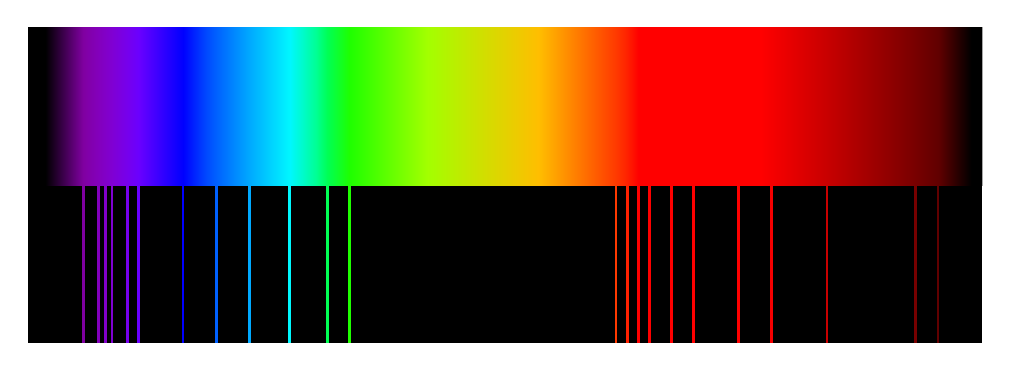
\begin{tikzpicture}[every node/.style={inner sep=0,outer sep=0}]
        \renewcommand*{\do}[1]{
            \storeRGBofWavelength{\Rval}{\Gval}{\Bval}{#1}
                \definecolor{wl#1}{rgb}{\Rval, \Gval, \Bval}
            }
        \docsvlist{370,372,375,378,395,400,402,405,408,415,420,440,450,455,470,488,500,505,515,550,600,635,640,645,650,660,670,690,700,705,730,750,770,780,795,800}
        % The manual of pgf says about \pgfshadepath, that it must a height and width of 100 bp
        % Strangely, here 50bp are enough
        \pgfdeclarehorizontalshading{spectrum}{100bp}{
            color(0bp)=(wl370); color((375-370)/430*50bp)=(wl375);
            color((378-370)/430*50bp)=(wl378); color((395-370)/430*50bp)=(wl395);
            color((400-370)/430*50bp)=(wl400); color((402-370)/430*50bp)=(wl402);
            color((405-370)/430*50bp)=(wl405); color((408-370)/430*50bp)=(wl408);
            color((415-370)/430*50bp)=(wl415); color((420-370)/430*50bp)=(wl420);
            color((440-370)/430*50bp)=(wl440); color((450-370)/430*50bp)=(wl450);
            color((455-370)/430*50bp)=(wl455); color((470-370)/430*50bp)=(wl470);
            color((488-370)/430*50bp)=(wl488); color((500-370)/430*50bp)=(wl500);
            color((505-370)/430*50bp)=(wl505); color((515-370)/430*50bp)=(wl515);
            color((550-370)/430*50bp)=(wl550); color((600-370)/430*50bp)=(wl600);
            color((635-370)/430*50bp)=(wl635); color((640-370)/430*50bp)=(wl640);
            color((645-370)/430*50bp)=(wl645); color((650-370)/430*50bp)=(wl650);
            color((660-370)/430*50bp)=(wl660); color((670-370)/430*50bp)=(wl670);
            color((690-370)/430*50bp)=(wl690); color((700-370)/430*50bp)=(wl700);
            color((705-370)/430*50bp)=(wl705); color((730-370)/430*50bp)=(wl730);
            color((770-370)/430*50bp)=(wl770); color((780-370)/430*50bp)=(wl780);
            color((795-370)/430*50bp)=(wl795); color((800-370)/430*50bp)=(wl800)
        }
        \fill (0,0) rectangle +(\textwidth,2);
        \foreach[evaluate={\x=(\wl-370)/430}] \wl in {372,375,378,395,402,405,408,415,420,440,455,470,488,505,515,635,640,645,650,660,670,690,705,730,770,780,795}
            \draw[line cap=rect, line width=1pt,wl\wl] (\textwidth*\x,0.5pt) -- +(0,2);
        \shade[shading=spectrum] (0,2) rectangle +(\textwidth,2);
    \end{tikzpicture}
\end{document}
